% Hlavicka pro protokoly z fyzikalniho praktika.
% Verze pro: LaTeX
% Verze hlavicky: 22. 2. 2007
% Autor: Ustav fyziky kondenzovanych latek
% Ke stazeni: www.physics.muni.cz/ufkl/Vyuka/
% Licence: volne k pouziti, nejlepe k vcasnemu odevzdani protokolu z Vaseho mereni.

\documentclass[a4paper,11pt]{article}

% Kodovani (cestiny) v dokumentu: utf-8
%\usepackage[cp1250]{inputenc}	% Omezena stredoevropska kodova stranka, pouze MSW.
\usepackage[utf8]{inputenc}	% Doporucujeme pouzivat UTF-8 (unicode).
\usepackage[T1]{fontenc}
\usepackage{lmodern}

%%% Nemente:
\usepackage[margin=2cm]{geometry}
\newtoks\jmenopraktika \newtoks\jmeno \newtoks\datum
\newtoks\obor \newtoks\skupina \newtoks\rocnik \newtoks\semestr
\newtoks\cisloulohy \newtoks\jmenoulohy
\newtoks\tlak \newtoks\teplota \newtoks\vlhkost
\usepackage{amsmath}
\usepackage{mathtools}
\usepackage{graphicx}
\usepackage{multirow}

\usepackage{pgfplotstable} 
\usepackage{booktabs}

\graphicspath{ {./images/} }
%%% Nemente - konec.


%%%%%%%%%%% Doplnte pozadovane polozky:

\jmenopraktika={Fyzikální praktikum 3}  % nahradte jmenem vaseho predmetu
\jmeno={Artem Gorodilov}            % nahradte jmenem mericiho
\datum={26. ~února  2024}        % nahradte datem mereni ulohy
\obor={Astrofyzika}                     % nahradte zkratkou vami studovaneho oboru
\skupina={Po 14:00}            % nahradte dobou vyuky vasi seminarni skupiny
\rocnik={II}                  % nahradte rocnikem, ve kterem studujete
\semestr={II}                 % nahradte semestrem, ve kterem studujete

\cisloulohy={C}               % nahradte cislem merene ulohy
\jmenoulohy={Studium termoelektronové emise} % nahradte jmenem merene ulohy

\tlak={979}                   % nahradte tlakem pri mereni (v hPa)
\teplota={21.4}               % nahradte teplotou pri mereni (ve stupnich Celsia)
\vlhkost={46}               % nahradte vlhkosti vzduchu pri mereni (v %)

%%%%%%%%%%% Konec pozadovanych polozek.


%%%%%%%%%%% Uzitecne balicky:
\usepackage[czech]{babel}
\usepackage{graphicx}
\usepackage{amsmath}
\usepackage{xspace}
\usepackage{url}
\usepackage{indentfirst}
\usepackage{listings}
\usepackage{subcaption}
\usepackage{caption}
\usepackage{tabularx}
\usepackage[labelformat=parens,labelsep=quad,skip=3pt]{caption}

%%%%%% Zamezeni parchantu:
\widowpenalty 10000 \clubpenalty 10000 \displaywidowpenalty 10000
%%%%%% Parametry pro moznost vsazeni vetsiho poctu obrazku na stranku
\setcounter{topnumber}{3}	  % max. pocet floatu nahore (specifikace t)
\setcounter{bottomnumber}{3}	  % max. pocet floatu dole (specifikace b)
\setcounter{totalnumber}{6}	  % max. pocet floatu na strance celkem
\renewcommand\topfraction{0.9}	  % max podil stranky pro floaty nahore
\renewcommand\bottomfraction{0.9} % max podil stranky pro floaty dole
\renewcommand\textfraction{0.1}	  % min podil stranky, ktery musi obsahovat text
\intextsep=8mm \textfloatsep=8mm  %\intextsep pro ulozeni [h] floatu a \textfloatsep pro [b] or [t]

% Tecky za cisly sekci:
\renewcommand{\thesection}{\arabic{section}.}
\renewcommand{\thesubsection}{\thesection\arabic{subsection}.}
% Jednopismenna mezera mezi cislem a nazvem kapitoly:
\makeatletter \def\@seccntformat#1{\csname the#1\endcsname\hspace{1ex}} \makeatother

\begin{document}

\thispagestyle{empty}

{
\begin{center}
\sf 
{\Large Ústav fyzikální elektroniky PřF MU} \\
\bigskip
{\huge \bfseries FYZIKÁLNÍ PRAKTIKUM} \\
\bigskip
{\Large \the\jmenopraktika}
\end{center}

\bigskip

\sf
\noindent
\setlength{\arrayrulewidth}{1pt}
\begin{tabular*}{\textwidth}{@{\extracolsep{\fill}} l l}
\large {\bfseries Zpracoval:}  \the\jmeno & \large  {\bfseries Naměřeno:} \the\datum\\[2mm]
\large  {\bfseries Obor:} \the\obor  \hspace{40mm}  {\bfseries Skupina:} \the\skupina %
%{\bfseries Ročník:} \the\rocnik \hspace{5mm} {\bfseries Semestr:} \the\semestr  
&\large {\bfseries Testováno:}\\
\\
\hline
\end{tabular*}
}

\bigskip

{
\sf
\noindent \begin{tabular}{p{3cm} p{0.6\textwidth}}
\Large  Úloha č. {\bfseries \the\cisloulohy:} \par
\smallskip
% $T=\the\teplota$~$^\circ$C \par
% $p=\the\tlak$~hPa \par
% $\varphi=\the\vlhkost$~\%
&\Large \bfseries \the\jmenoulohy  \\[2mm]
\end{tabular}
}

\vskip10pt
    \begin{minipage}[t]{0.5\textwidth} 
        \section{Zadání}    
            \begin{enumerate}
                \item Změřit, jak se anodový proud mění v závislosti na anodovém napětí $I_a$ = $f(U)$, kde $U$ je v rozmezí od -5 V do 500 V, pro dvě hodnoty žhavicího proudu $I_f$. Výsledné závislosti zobrazit v grafu.
                \par Zobrazit náběhovou oblast anodového proudu $I_a$ v grafu s použitím souřadnic $\ln I_a$ = $f(U_a)$ a určit teplotu elektronů.
                \par Zpracovat oblast nasyceného anodového proudu $I_{nas}$ = $f(U)$ pro $U$ < 500 V do grafu v souřadnicích $\ln I_{nas}$ = $\sqrt{U_a}$ a určit přírůstek proudu způsobený Schottkyho efektem.
                
                \item Určit anodové napětí $U_a$, při kterém je anodový proud nasycený, tj. $I_a = I_{nas}$.
                
                \item Měřením závislosti nasyceného anodového proudu na žhavícím proudu $I_{nas} = f(I_f)$ určit výstupní práci wolframu $w$ pomocí Richardsonovy-Dushmanovy rovnice.
            \end{enumerate}
        \section{Teorie}
            \subsection{Termoelektronová emise}
                Experiment se zabývá uvolňováním elektronů z kovových povrchů, které je vyvoláno jejich zahřátím na vysokou teplotu. Tento jev, známý jako termoemise, nám umožňuje získat informace o vazebných silách, kterými jsou elektrony drženy v kovech.
                \par Když je kov zahřát na dostatečně vysokou teplotu, začne emitovat elektrony. Avšak, aby mohly elektrony opustit povrch kovu, musí mít jejich energie vyšší hodnotu než je tzv. výstupní práce kovu $w$. Celkový proud elektronů uvolněných z kovu při teplotě $T$ a s výstupní prací $w$ je popsán jako nasycený emisní proud:
    \end{minipage}
    \hspace{10pt}
    \begin{minipage}[t]{0.5\textwidth} 
                \begin{equation}
                    I_{\text{nas}} = B T^2 \exp\left(-\frac{w}{kT}\right)
                \end{equation}
                kde $B$ je konstanta zahrnující plochu katody a termoemisní konstantu a $k$ je Boltzmannova konstanta. Po logaritmování a úpravě dostáváme vztah pro Richardsonovu-Dushmanovu přímku:
                \begin{equation}
                    y = -\frac{w}{k}x + \ln B
                \end{equation}
                kde $y = \ln (I_{nas}/T^2)$ a $x = 1/T$.
                \par Teplotu vlákna určíme z měření žhavícího proudu $I_f$ a napětí $U_f$:
                \begin{equation}
                    R_t = \frac{U_f}{I_f} = \frac{\rho d }{S} (1+ \alpha t)
                \end{equation}
                kde $R_t$ je odpor vlákna při teplotě $t$, $\rho$ je hustota materiálu, $d$ je průměr vlákna, $S$ je jeho plocha a $\alpha$ je teplotní součinitel odporu.
                \par Zajímavostí je, že při snižování anodového napětí se elektrony stávají více brzděny elektrickým polem.

                \vspace{10pt}   
                \par \centering
                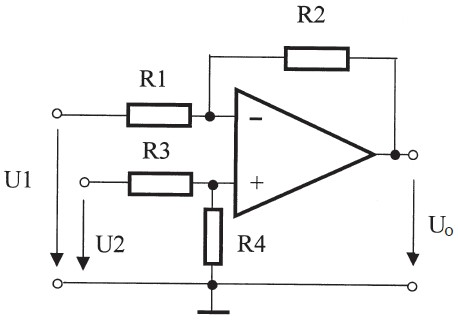
\includegraphics[scale=0.6]{rozd}
                \captionsetup{justification=centering, font=footnotesize}
                \captionof{figure}{a - integrální, b - diferenciální tvar rozdělení energie elektronů. Oblast c je oblast je oblast nábojového proudu, oblast d je oblast saturačního proudu.}
                \label{fig:dif}
                \vspace{10pt}
                \raggedright                
    \end{minipage}
\newpage
    \begin{minipage}[t]{0.5\textwidth} 
                \par Pro naběhovou oblast platí, že anodový proud $I_a$ je exponenciálně závislý na anodovém napětí $U_a$ a teplotě emitovaných elektronů $T_e$:
                \begin{equation}
                    I_a = I_0 \exp\left(\frac{eU_a}{kT_e}\right)
                \end{equation}
            \subsection{Schottkyho efekt}
                Pokud se katoda nachází v silném elektrickém poli, dochází ke snížení výstupní práce katody, což můžeme popsat následujícím vztahem:
                \begin{equation}
                    w_p = \sqrt{\frac{e^3E}{4\pi \epsilon_0}}
                \end{equation}
                kde $e$ je náboj elektronu, $\epsilon_0$ je permitivita vakua a $E$ je intenzita elektrického pole u povrchu katody.
                \par A tedy nová hodnota $w_p$ výstupní práce bude:
                \begin{equation}
                    w = w - w_p = w - \sqrt{\frac{e^3E}{4\pi \epsilon_0}}
                \end{equation}
                \par Schottkyho efekt je schematicky znázorněn na obrázku (2).
                
                \vspace{10pt}           
                \par \centering
                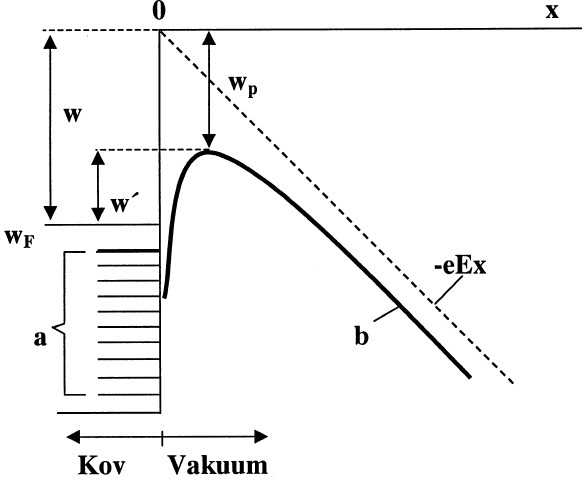
\includegraphics[scale=0.5]{schot}
                \captionsetup{justification=centering, font=footnotesize}
                \captionof{figure}{Schottkyho efekt.}
                \label{fig:dif}
                \vspace{10pt}
                \raggedright 
                
                \par Nasycený anodový proud pak bude záviset na intenzitě elektrického pole u povrchu katody a vystupní práci: 
                \begin{equation}
                    \ln I_{nas}' = \ln I_{nas} + \sqrt{\frac{e^3}{4\pi \epsilon_0 k^2 T^2}} \sqrt{E}
                \end{equation}
                \par Intenzitu elektrického pole u žhavené katody lze určit ze vztahu:
                \begin{equation}
                    E = U_a \frac{L-D}{D} \frac{1}{r \ln(R/r)}
                \end{equation}
                kde $L$, $D$, $R$ a $r$ jsou geometrické parametry katody a anody, specifické pro použité zařízení.
    \end{minipage}
    \hspace{10pt}
    \begin{minipage}[t]{0.5\textwidth} 
        \section{Měření}  
                Experiment provádíme s poloautomatickým nastavením, kde jsou všechna napětí a měřicí zařízení připojena k počítači, což nám umožňuje okamžité grafické znázorňování získaných dat.
                \par Tímto způsobem můžeme ihned po zaznamenání dat identifikovat oblast náběhového proudu.
                \par Za tímto účelem zjistíme závislost $\ln I_a$ = $f(U_a)$o případech dvou $I_f$ = 1.8 A a $I_f$ = 1.9 A. Poté získané údaje vyneseme do grafu a provedeme lineární fitování oblasti náběhového proudu. Poté ze vzorce (3) určíme teplotu emitovaných elektronů T pomocí získané směrnice přímky $\alpha$ jako $T = \frac{e}{k \alpha}$. Výsledky jsou znázorněny na obrázku (3).
                \par Z toho dostáváme následující teploty emitovaných elektronů: 
                \begin{center}
                    $T_{1.8}$ = (4080 $\pm$ 340) K ~ a ~ $T_{1.9}$ = (4650 $\pm$ 320) K
                \end{center}
                
                \vspace{10pt}           
                \par \centering
                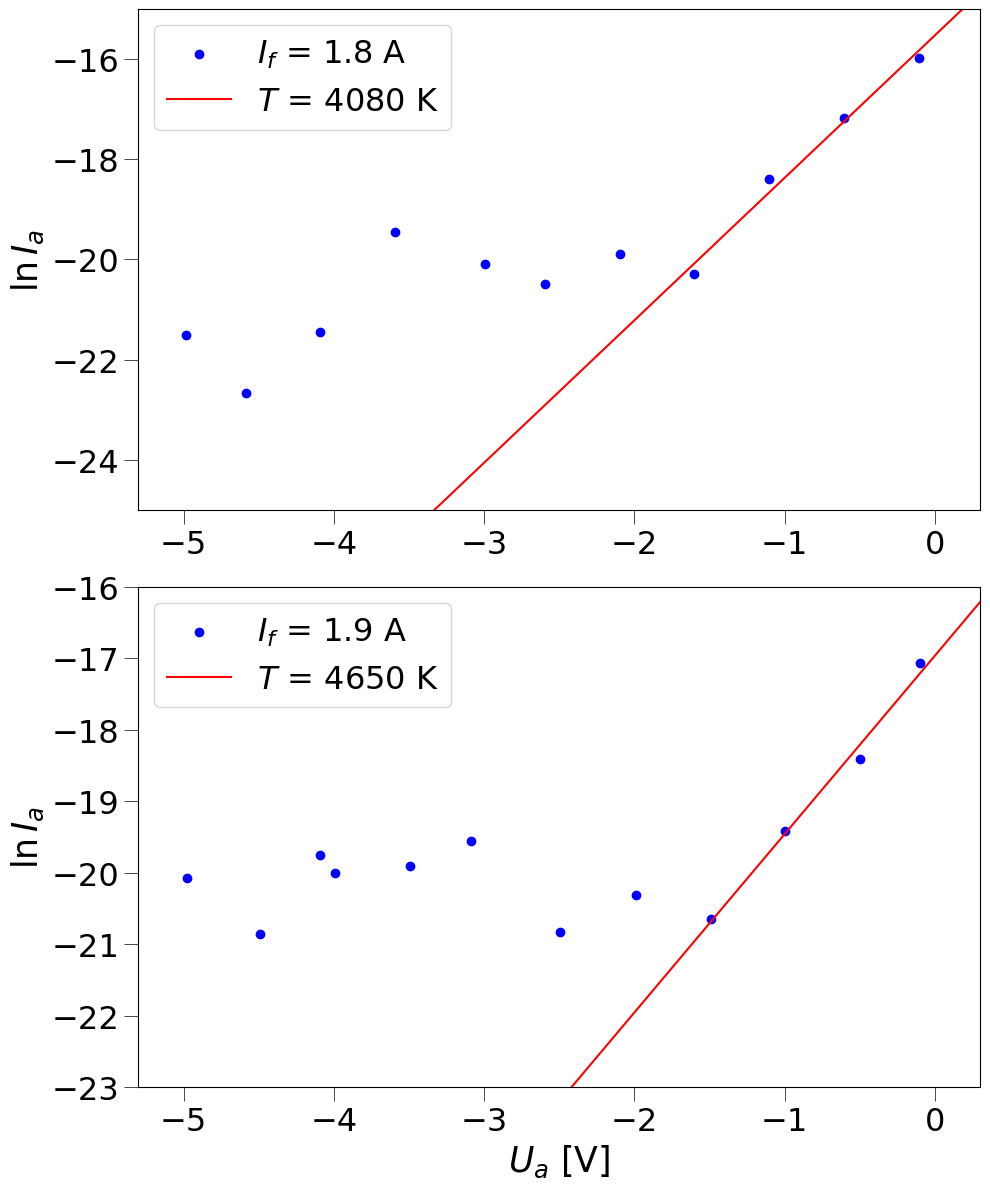
\includegraphics[scale=0.3]{nabeh}
                \captionsetup{justification=centering, font=footnotesize}
                \captionof{figure}{Závislost $\ln I_a$ = $f(U_a)$ pro $I_f$ = 1.8 A a $I_f$ = 1.9 A.}
                \label{fig:dif}
                \vspace{10pt}
                \raggedright 

                \par Dále uvažujeme oblast nasyceného proudu. Nejprve zjistíme závislost $\ln I_{nas}$ = $\sqrt{U_a}$ a vykreslíme data. Data jsou znázorněna na obrázku (4). 
                \par Poté z grafu ručně určíme hodnotu přírůstku proudu. Získáme následující naměřené hodnoty: 
                \begin{center}
                    $\Delta I_{nas, 1.8}$ = 4.75(1) $\mu$A
                    \vspace{5pt}
                    \par $\Delta I_{nas, 1.9}$ = 13.36(1) $\mu$A
                \end{center}
    \end{minipage}
\newpage
    \begin{minipage}[t]{0.5\textwidth}
                \vspace{10pt}           
                \par \centering
                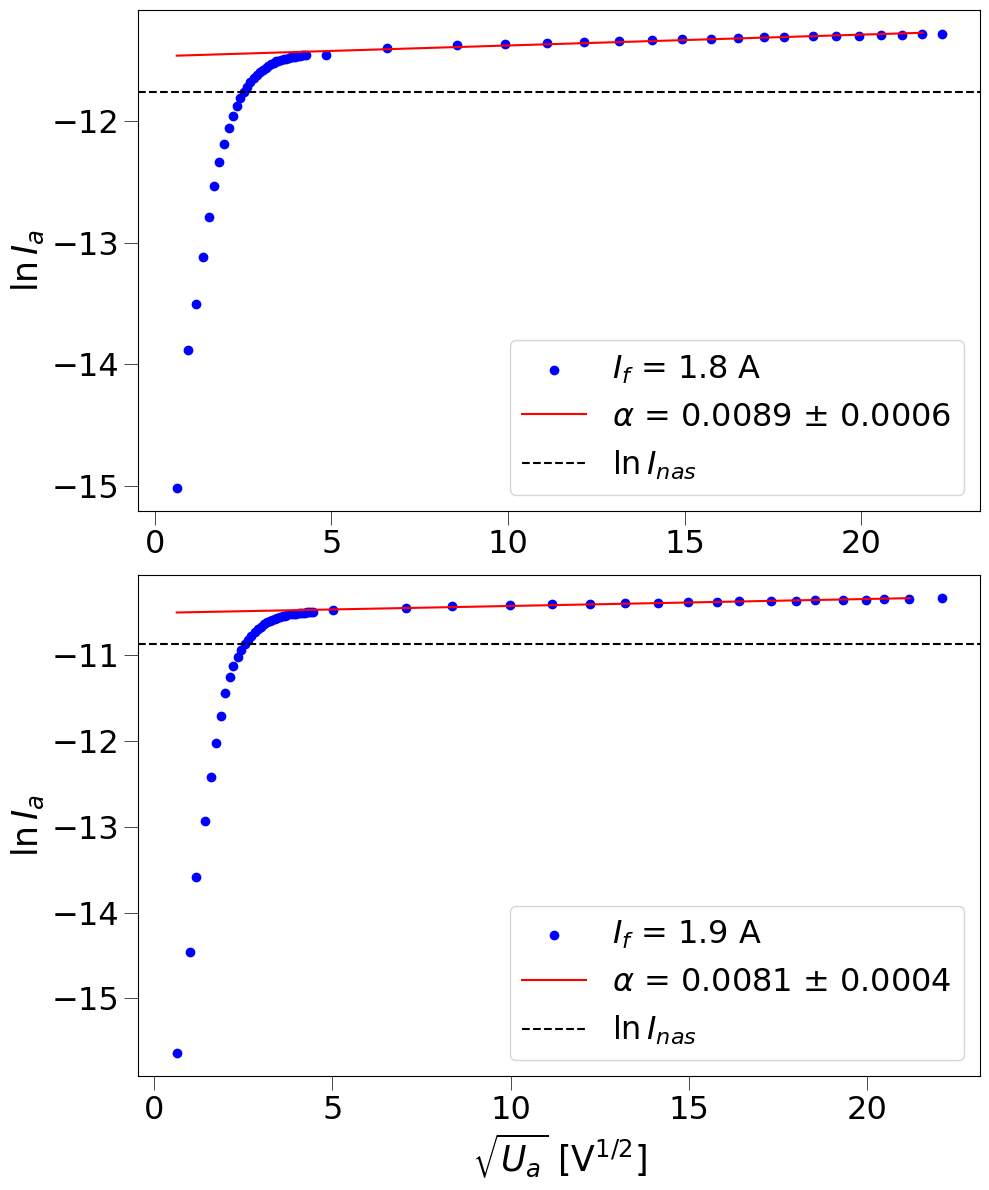
\includegraphics[scale=0.32]{nas}
                \captionsetup{justification=centering, font=footnotesize}
                \captionof{figure}{Závislost $\ln I_{nas}$ = $\sqrt{U_a}$ pro $I_f$ = 1.8 A a $I_f$ = 1.9 A.}
                \label{fig:dif}
                \vspace{10pt}
                \raggedright 

                Podle vzorce (7) určete intenzitu elektrického pole v blízkosti katody pro anodové napětí pri kterém je anodový proud nasycený: 
                \begin{center}
                    $U_{a, 1.8}$ = 6.4 V ~ a ~ $U_{a, 1.9}$ = 6.48 V
                \end{center}
                \begin{center}
                    $E$ = 1.25 $\cdot$ 10$^6$ V/m
                \end{center}

                \par Podle vzorce (6) tedy zjistíme teoretickou hodnotu přírůstku proudu: 
                \begin{center}
                    $\Delta I_{nas, teor, 1.8}$ = 8.80(9) $\mu$A
                    \vspace{5pt}
                    \par $\Delta I_{nas, teor, 1.9}$ = 21.1(2) $\mu$A
                \end{center}
                
                Dale změříme závislost nasyceného anodového proudu na žhavícím proudu $I_{nas} = f(I_f)$ pro napětí $U_a$ = 19.95 V.
                \par Pomocí vzorce (3) určíme teplotu vlákna $t$. Poté vypočteme zavislost $\ln (I_{nas}/T^2)$ = $f(1/T)$ a vyneseme data do grafu. Data jsou znázorněna na obrázku (5). 
                \par Z lineárního fitování získáme hodnotu výstupní práce $w$ wolframu a konstantu zahrnující plochu katody a termoemisní konstantu $B$:
                \begin{center}
                    $w$ = 3.55(6) eV
                    \vspace{5pt}
                    \par $B$ = 1.1(6) $\cdot$ 10$^6$ A/K$^{-2}$
                \end{center}
    \end{minipage}
    \hspace{10pt}  
    \begin{minipage}[t]{0.5\textwidth} 
                \vspace{10pt}           
                \par \centering
                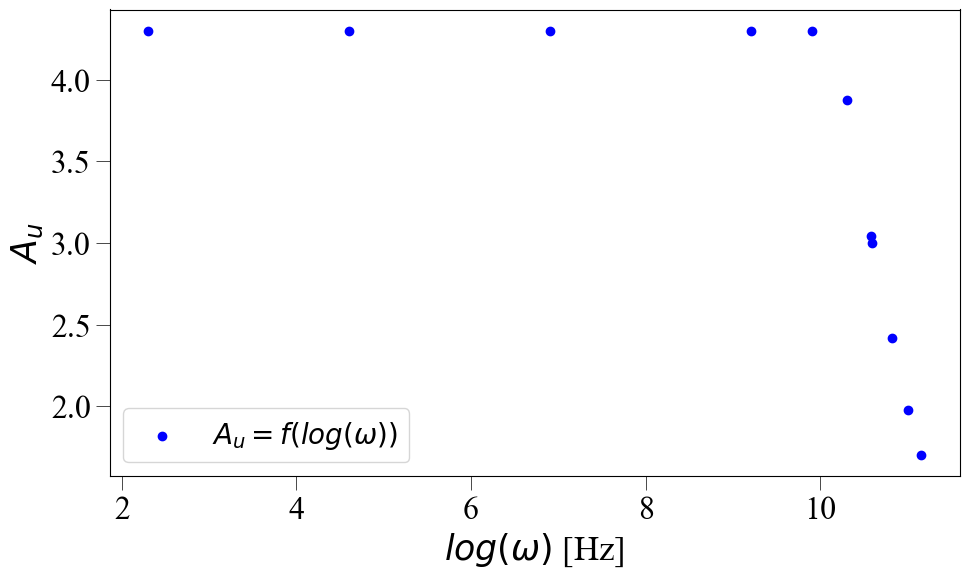
\includegraphics[scale=0.32]{R-D}
                \captionsetup{justification=centering, font=footnotesize}
                \captionof{figure}{Závislost $\ln (I_{nas}/T^2)$ = $f(1/T)$ pro $U_a$ = 19.95 V. R-D křivka.}
                \label{fig:dif}
                \vspace{10pt}
                \raggedright 
       
                \par Tabulkové hodnoty použité při výpočtu:
                \begin{center}
                    \begin{tabular}{ll}
                        $e$ = 1.6 $\cdot$ 10$^{-19}$ C & $k$ = 1.38 $\cdot$ 10$^{-23}$ J/K \\
                        $\epsilon_0$ = 8.85 $\cdot$ 10$^{-12}$ F/m & $\rho$ = 4.89 $\cdot$ 10$^{-8}$ $\Omega$m \\
                        $\alpha$ = 4.83 $\cdot$ 10$^{-3}$ K$^{-1}$ & $r$ = 0.045 mm \\
                        $R$ = 17 mm & $L$ = 25 mm \\
                        $D$ = 15 mm & $d/s$ = 7.76 $\cdot$ 10$^{6}$ m
                    \end{tabular}
                \end{center}
                \par Výsledky měření jsou v tabulce (1) a (2).
                \vspace{10pt}
                \par K výpočtu veličin a jejich nejistot byla použita knihovna Uncertinties pro Python: \href{pypi.org/project/uncertainties}. Chyby byly rozšířeny o Studentův koeficient (2-Tail Confidence Level) s ohledem na stupně volnosti pro každou hodnotu, pro interval spolehlivosti 68.27\%.
        \section{Závěr}  
                Ze získaných dat jsme určili teplotu emitovaných elektronů $T_{1.8}$ = (4080 $\pm$ 340) K a $T_{1.9}$ = (4650 $\pm$ 320) K pro $I_f$ = 1.8 A a $I_f$ = 1.9 A resp. Vidime, že teplota elektronů se zvyšuje s žhavícím proudem.
                \par Dále jsme určili hodnotu přírůstku proudu pro napětí $U_a$ = 500 V, které odpovídá intenzitě elektrického pole $E$ = 1.25 $\cdot$ 10$^6$ V/m. Získané hodnoty $\Delta I_{nas, 1.8}$ = 7.907(9) $\mu$A a $\Delta I_{nas, 1.9}$ = 19.22(1) $\mu$A. Vidíme, že naměřené hodnoty se liší od teoretických hodnot o 40\% a 30\% resp. 
                \par Anodové napětí, při kterém je anodový proud nasycený, jsme určili jako $U_{a, 1.8}$ = 6.4 V a $U_{a, 1.9}$ = 6.48 V.
                \par Nakonec jsme určili výstupní práci wolframu $w$ = 3.55(6) eV a konstantu zahrnující plochu katody a termoemisní konstantu $B$ = 1.1(6) $\cdot$ 10$^6$ A/K$^{-2}$. Ziskaná hodnota výstupní práce se liší od tabulkové hodnoty $w_{tab}$ = 4.5 eV o 21\%.  To bylo s největší pravděpodobností způsobeno tím, že jsme při měření $I_f$ použili rozsah 1.8 A až 1.9 A. Hodnota výstupní práce by byla přesnější, kdybychom při měření použili větší interval proudu. 
    \end{minipage}
\newpage
    \begin{center}
        \section{Přílohy}
            \subsection{Tabulka naměřených a vypočtených hodnot pro $I_f$ = 1.8 A}
                \begin{minipage}[t]{0.48\textwidth} % Adjust the width as needed
                    \vspace{0pt}
                    \pgfplotstabletypeset[
                        col sep=comma,
                        string type,
                        every head row/.style={before row=\toprule, after row=\midrule},
                        columns/U_f/.style={column name=U_f [V]},
                        columns/I_f/.style={column name=I_f [A]},
                        columns/U_a/.style={column name=U_a [V]},
                        columns/I_a /.style={column name=I_a [$\mu$ A]},
                        columns/lnI_a/.style={column name=\ln I_a},
                        columns/sqrtU_a/.style={column name=\sqrt{U_a}},
                        skip rows between index={0}{34},
                    ]{data/I_18_out.csv}  
                \end{minipage}%
                \hspace{10pt}  
                \begin{minipage}[t]{0.48\textwidth} % Adjust the width as needed
                    \vspace{0pt}
                    \pgfplotstabletypeset[
                        col sep=comma,
                        string type,
                        every head row/.style={before row=\toprule, after row=\midrule},
                        columns/U_f/.style={column name=U_f [V]},
                        columns/I_f/.style={column name=I_a [A]},
                        columns/U_a/.style={column name=U_a [V]},
                        columns/I_a /.style={column name=I_a [$\mu$ A]},
                        columns/lnI_a/.style={column name=\ln I_a},
                        columns/sqrtU_a/.style={column name=\sqrt{U_a}},
                        skip rows between index={35}{70},
                    ]{data/I_18_out.csv} 
                \end{minipage}
    \end{center}
\newpage    
            \begin{center}
                \subsection{Tabulka naměřených a vypočtených hodnot pro $I_f$ = 1.9 A}
                    \begin{minipage}[t]{0.48\textwidth} % Adjust the width as needed
                        \vspace{0pt}
                        \pgfplotstabletypeset[
                            col sep=comma,
                            string type,
                            every head row/.style={before row=\toprule, after row=\midrule},
                            columns/U_f/.style={column name=U_f [V]},
                            columns/I_f/.style={column name=I_f [A]},
                            columns/U_a/.style={column name=U_a [V]},
                            columns/I_a /.style={column name=I_a [$\mu$ A]},
                            columns/lnI_a/.style={column name=\ln I_a},
                            columns/sqrtU_a/.style={column name=\sqrt{U_a}},
                            skip rows between index={0}{34},
                        ]{data/I_19_out.csv}  
                    \end{minipage}%
                    \hspace{10pt}  
                    \begin{minipage}[t]{0.48\textwidth} % Adjust the width as needed
                        \vspace{0pt}
                        \pgfplotstabletypeset[
                            col sep=comma,
                            string type,
                            every head row/.style={before row=\toprule, after row=\midrule},
                            columns/U_f/.style={column name=U_f [V]},
                            columns/I_f/.style={column name=I_f [A]},
                            columns/U_a/.style={column name=U_a [V]},
                            columns/I_a /.style={column name=I_a [$\mu$ A]},
                            columns/lnI_a/.style={column name=\ln I_a},
                            columns/sqrtU_a/.style={column name=\sqrt{U_a}},
                            skip rows between index={35}{69},
                        ]{data/I_19_out.csv} 
                    \end{minipage}
            \end{center}
\newpage
            \begin{center}
                \subsection{Tabulka naměřených a vypočtených hodnot pro $U_a$ = 19.95 V} 
                    \pgfplotstabletypeset[
                        col sep=comma, % Defines the separator, comma for CSV
                        string type, % Treats columns as strings (not math mode)
                        every head row/.style={before row=\toprule,after row=\midrule},
                        every last row/.style={after row=\bottomrule},
                        columns/U_f/.style={column name=U_f [V]},
                        columns/I_f/.style={column name=I_f [A]},
                        columns/U_a/.style={column name=U_a [V]},
                        columns/I_a /.style={column name=I_a [$\mu$ A]},
                        columns/R/.style={column name=R_f [$\Omega$]},
                        columns/T/.style={column name=T [K]},
                        columns/x/.style={column name=x [1/K]},
                        columns/y/.style={column name=y},
                    ]{data/I_I_out.csv} 
            \end{center}
\end{document}